\Chapter{SQL lekérdezések végrehajtása}

\Section{Execution Plan}

A lekérdezés végrehajtási terv elkészítésével információkat nyerhetünk a lekérdezések hatékonyságáról. Ennek segítségével optimalizálhatjuk például egy olyan weboldal működését, mely sok és bonyolultabb lekérdezést végez adatbázisból. A hatékonyságot általában indexek hozzáadásával vagy elvételével illetve a táblák kapcsolási sorrendjének módosításával vagy kocsolási módjának megváltoztatásával segíthetjük elő.

\Section{Az \texttt{EXPLAIN} parancs}

A MySQL adatbázismotorban az Executing Plan hez szükséges információkat az EXPLAIN parancsal használatával kaphatjuk meg.
A parancs megfelelő utasítással együtt használva (SELECT, DELETE, INSERT, REPLACE, UPDATE)  információkat jelenít meg az optimalizáló által előállított feldolgozási tervről. Láthatóvá válik például a táblák összekapcsolási sorrendje.

További információk érhetők el a SHOW WARNINGS használatával.
A FORMAT parancs használható kimeneti formátum választásra. TRADITIONAL az alapértelmezett táblázatos alak. JSON pedig JSON formátumban jeleníti meg a kimenetet.

A parancs használata rávilágít arra, hol van szükség indexek használatára a lekérdezés gyorsítására, illetve ellenőrizhetjük, hogy a táblák megfelelő sorrendben vannak e összekapcsolva. 
JOIN helyett STRAIGHT\_JOIN használatával tippek adhatóak az optimalizálónak, a táblák kapcsolási sorrendkéről. De a STRAIGHT\_JOIN letiltja a semijoin transzformációkat, így indexelés ebben az esetben nem használható.
ANALYZE TABLE paranccsal frissíthetőek a statisztikák, mint a kulcsok számossága. Ez befolyásolhatja az optimalizáló döntéseit. 

% TODO: Ide érdemes kifejteni, MySQL Workbench-es példákkal illusztrálni, hogy hogyan működik a parancs.

\Section{Teszt adatbázis megtervezése}

Az execution plan optimalizálási módnál a kapott információk felhasználásával tudjuk optimalizálni a lekérdezéseket.
Olyan adatbázist kell választanunk ennek kipróbáláshoz amelyben használhatók indexek de nincs feltétlen szükség rájuk, össze kapcsolhatunk több táblát és rendezhetjük az adatokat például növekvő sorrendben. 

\begin{figure}[h!]
\centering
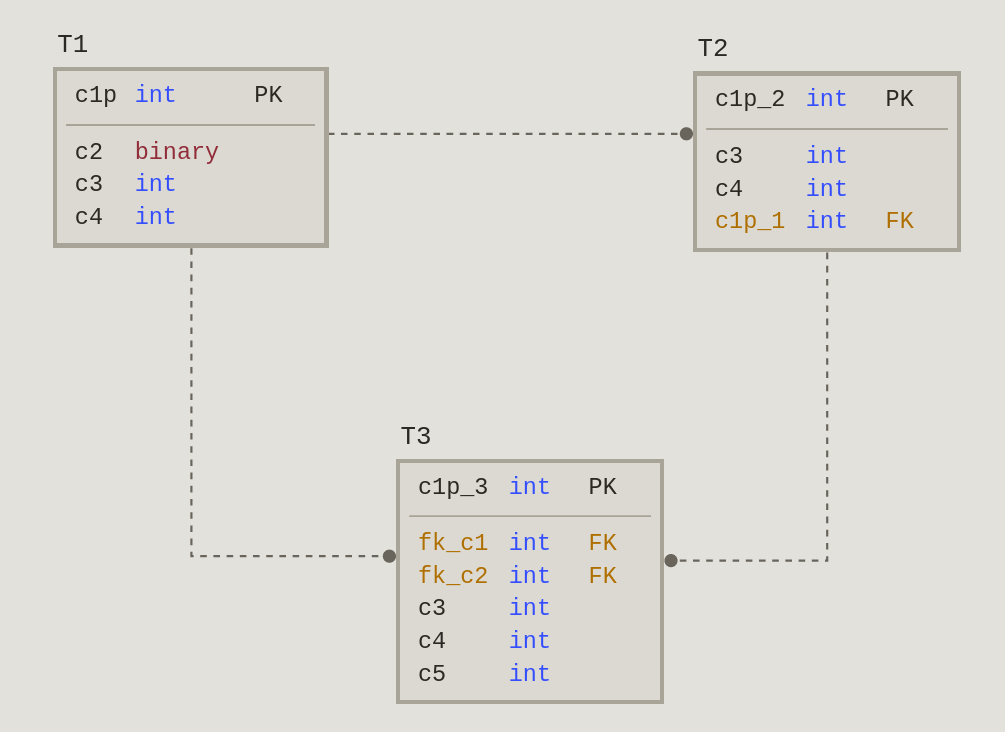
\includegraphics[width=\textwidth]{images/schema.png}
\caption{Adatbázis séma}
\label{fig:schema}
\end{figure}

Az oszlopnevek számozottak. A \texttt{c3}-\texttt{c5} Az értékeik véletlenszerűen generált egészek, \texttt{c3} $in [0, 100]$, \texttt{c4} $in [0, 10000]$, \texttt{c5} $in [0, 10]$.

T1 kitöltése minta:
\begin{python}
INSERT INTO `testdb`.`T1` (`c1p`, `c2`, `c3`, `c4`)
VALUES ('0', '1', '50', '150');
\end{python}
